\documentclass[11pt,a4paper]{article}
\usepackage[left=20mm,right=15mm,top=15mm,bottom=15mm]{geometry}
\usepackage[utf8x]{inputenc}
\usepackage[L7x]{fontenc}
\usepackage[lithuanian]{babel}
\usepackage{amsmath}
\usepackage{tikz}
\usepackage{pgfplots}
\usepackage{graphicx}
\usetikzlibrary{patterns}

\begin{document}
\begin{titlepage}
  
  \begin{center}
    \textsc{\LARGE Vilniaus Gedimino Technikos universitetas}\\[2mm]
    \textsc{\Large Verslo vadybos fakultetas}\\[2mm]
    \textsc{\Large Įmonių ekonomikos ir vadybos katedra}\\[70mm]
    \textsc{\normalsize Ekonomikos kursinio darbo užduotis}\\[5mm]
    \textsc{\Large AB "Lietuvos dujos" įmonės gamybos išteklių produktyvumo analizė}\\[40mm]

    \begin{minipage}{1\textwidth}
      \begin{flushright}
        \emph{Darbą atliko:} EI-08/2 gr. studentas\\ Maksim Norkin\\
        \emph{Darbą tikrino:} $\_ \_ \_ \_ \_ \_ \_ \_ \_ \_ \_ \_ \_ \_ \_$\\
      \end{flushright}
    \end{minipage}
    \vfill
    {\large Vilnius \\ \the\year}
  \end{center}
\end{titlepage}
\setcounter{page}{2}
\tableofcontents
\newpage

\section*{Įvadas}
\addcontentsline{toc}{section}{Įvadas}

Energetika yra labai svarbus mūsų šiuolaikinės visuomenės pagrindas. Vienas iš 
esminių energetikos šaltinių yra kuras. Dažniausiai kaip efektyviai dirba
šalies energetinės sistemos, priklauso jos ekonominė padėtis, nes kuo 
greičiau vystosi ekonomika - tuo didesnė apkrova tenka energetinėms sistemoms.\\

Užsidarius Ignalinos AE, pagrindinis energetikos išteklius Lietuvoje jau nebebus 
elektros energija. Ją pakeis dujos. Dujos suks turbinas. Dėl to labai svarbu 
išsiaiškinti kokia yra AB "Lietuvos dujos" padėtis ekonominėje srityje.\\\\
\textbf{Darbo tikslas:} įvertinti įmonės AB "Lietuvos dujos" produktyvumą.\\
\textbf{Darbo uždaviniai:} 
\begin{itemize}
	\item Pamatyti AB "Lietuvos dujos" įmonės situaciją Lietuvos rinkoje;
	\item Detaliau susipažinti su įmonės darbo struktūra;
	\item Išanalizuot AB "Lietuvos dujos" darbo našumą;
	\item Išsiaiškinti įmonės vieno darbininko išdirbį;
	\item Taip pat panagrinėti įmonės kapitalo struktūra, bei išsiaiškinti kokia yra
	įmonės pakeičiamumo norma;
\end{itemize}
\textbf{Tyrimo laikotarpis:} 2007 - 2009 metai.\\

\newpage

\section{Gamybos šakos apimtys už 3 metus}

AB "Lietuvos dujos" operuoja tik dujomis, todėl norint sužinoti kiek aplamai 
Lietuvoje buvo sunaudota dujų, pasitelkime Lietuvos Statistikos departamento 
suteiktais duomenimis už 2009-2007 metus. Gaila, bet LS departamentas už 2009 
metus duomenų nepateikia.\\\\
\textsl{1.1 lentelė. Gamybos šakos apimtys už 3 metus. Informacija parinkta iš 1 
literatūros šaltinio.}\\
\begin{tabular}{|p{5cm}|p{3cm}|p{3cm}|p{3cm}|} \hline
	{Veiklos rodikliai} & {2009} & {2008} & {2007} \\ \hline
	Gamtinės dujos, mln. $m^3$ & - & 3 244.9 & 3 615.1 \\ \hline
\end{tabular}\\\\
Kaip matome, gamybos veiklos apimtys yra labai didelės. Duomenų vaizdingumui 
pateikiame grafiką.

\begin{center}
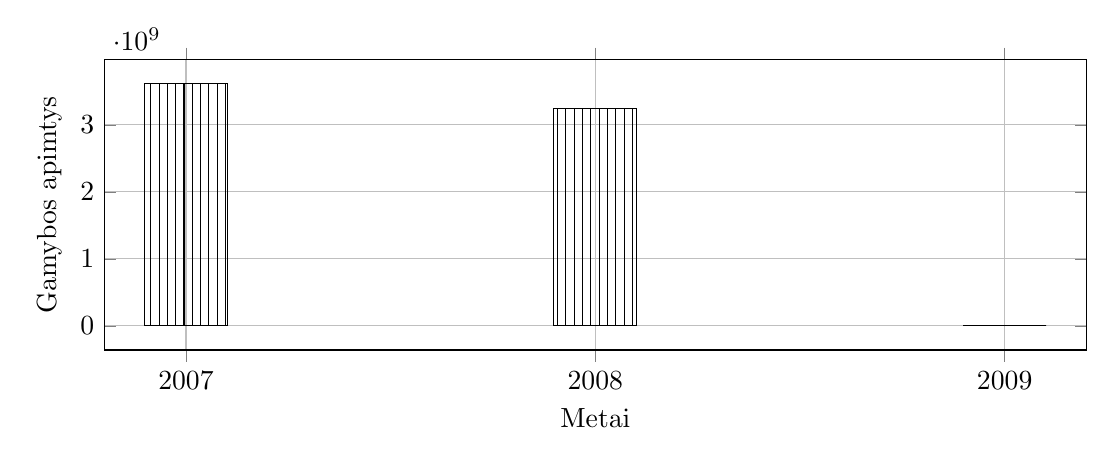
\begin{tikzpicture}
	\begin{axis}[
		x tick label style={
			/pgf/number format/1000 sep=
		},
		xtick = data,
		ybar,
		bar width=30pt,
		xlabel={Metai},
		ylabel={Gamybos apimtys},
		width=400pt,
		height=150pt,
		grid=major,
	]
		\addplot+[draw=black, pattern=vertical lines,] coordinates {
			(2009, 0)
			(2008, 3244.9e6)
			(2007, 3615.1e6)
		};
	\end{axis}
\end{tikzpicture}
\end{center}
\textsl{1.1 pav. Gamybos šakos apimtys.}\\

Iš grafikos ir skaičių matome, jog gamybos apimtys 2007 metais yra didesnės už 
2008 metų gamybos apimtis. Tai galėjo lemti 2008 metais padidėję mokesčiai už 
dujas.

2009 m. gamtines dujas į Lietuvą importavo penkios įmonės - AB "Lietuvos dujos" (LD), 
AB "Achema", UAB "Dujotekana", UAB "Kauno termofikacijos elektrinė" ir UAB "Haupas". 
Iš viso 2009 m. į Lietuvą importuota 2.7 mlrd. $m^3$ gamtinių dujų. UAB "Haupas" 
gamtines dujas importavo ne per Bendrovės dujų sistemą.\\

\includegraphics[width=400pt]{gamtiniu_duju_importo_struktura_lietuvoje_2009.png}\\
\textsl{2.1 pav. Gamtinių dujų importo struktūra Lietuvoje 2009 m.}\\

2009 m. gamtines dujas buitiniams ir nebuitiniams Lietuvos vartotojams tiekė LD, 
UAB "Fortum Joniškio energija", UAB "Druskininkų dujos", AB agrofirma "Josvainiai" 
ir UAB "Integras". UAB "Dujotekana" ir UAB "Haupas" dujas tiekė tik nebuitiniams 
vartotojams. AB "Achema" ir UAB "Kauno termofikacijos elektrinė" dujas importavo 
savo reikmėms.

\section{Įmonės apžvalga toje šakoje}

\subsection{Vizija ir misija}
AB "Lietuvos dujos" vizija - tapti geriausia energetikos sektoriaus kompanija.\\

Tai akcinė bendrovė planuoja pasiekti:
\begin{itemize}
	\item Būdami skaidria, patikima ir patrauklia vartotojams, socialiai atsakinga kompanija.
	\item Didinant kompanijos vertę.
	\item Pritraukdama, išlaikydama ir ugdydama geriausius darbuotojus.
	\item Optimizuodama kaštus, užtikrindama tinkamą investicijų gražą.
	\item Plėsdama savo veiką į naujus segmentus.
	\item Plėsdama savo infrastruktūrą (dujų sistemas).
	\item Užtikrindama aukštą IT, techninį ir technologinį lygį.
\end{itemize}

AB "Lietuvos dujos" misija - saugiai ir patikimai tiekti gamtines dujas, kad visiems gyventi būtų patogiau.

\subsection{Įmonės veikla}

Pagrindinė AB "Lietuvos dujos" veikla - gamtinių dujų pirkimas (importas) ir pardavimas klientams, perdavimo,
skirstymo paslaugų tiekimas, racionalus Lietuvos gamtinių dujų tiekimo infrastruktūros, kurios dauguma priklauso 
bendrovei, vystymas. AB "Lietuvos dujos" iš viso eksploatuoja 1.9 tūkst. km magistralinių ir 8.1 tūkst. km skirstomųjų 
dujotiekių. Bendrovė dujas tiekia energetikos, pramonės, žemės ūkio įmonėms, smulkiojo komercinio sektoriaus 
vartotojams ir gyventojams. Bendrovė tranzitu gamtines dujas tiekia į Rusijos Federacijos Kaliningrado sritį.
Turi 550 tūkst. klient, įmonėje dirba 1800 darbuotojų.\\

Bendrovė perėmė ir tęsia nuo 1961 metų Lietuvoje vykdomą gamtinių dujų verslą. Akcine bendrove įregistruota 1995 metais.
Įmonė privatizuota dviem etapais. Jos akcininkas viešojo konkurso tvarka tapo pasaulio masto energetikos kompanijos:
2002 metais 34\% akcijų paketą įsigijo "Ruhrgas AG" ir "E.ON Energie AG" (Vokietija) konsorciumas (dabar akcijas
valdo "E.ON Ruhrgas International AG") ir 2004 metais - 34\% akcijų įsigijo gamtinių dujų tiekėja OAO "Gazprom" (Rusija).\\

"E.ON Ruhrgas International AG" - valdymo bendrovė, kuri yra sudėtinė "E.ON AG" dalis. "E.ON AG" yra viena didžiausių
pasaulyje elektros, dujų, komunalinių paslaugų bei atsinaujinančios energijos gamybos bendrovė.\\

OAO "Gazprom" yra pasaulinė energetikos bendrovė, vykdanti dujų ir kitų angliavandenilių mišinių geologinius
tyrimus, gamybą, transportavimą, laikymą, perdirbimą ir pardavimą, taip pat elektros energijos ir šiluminės
energijos gamyba ir tiekimą. OAO "Gazprom" turi didžiausias pasaulyje patvirtintas gamtinių dujų atsargas.\\

\subsection{Organizacinė struktūra}

Įmonės organizacinė struktūra:\\

Visuotinis akcininkų susirinkimas
\begin{itemize}
	\item Valdyba. Dr. Valery Golubev (pirmininkas), Dr.Achim Saul (pirmininko pavaduotojas), Jorg Tumat, Kirill Seleznev
	\begin{itemize}
		\item Vadovybė. Viktoras Valentukevičius (generalinis direktorius), Dr. Joachim Hockertz, Vladimir Obukhob, Jonas Janiulionis, Giedrė Glinskienė
		\begin{itemize}
			\item Filialai
			\begin{itemize}
				\item Funkcijos: skirstymo sistemos operatorius
			\end{itemize}
			\item Valdymo ir dujų perdavimo centras
			\begin{itemize}
				\item Funkcijos: valdymas, perdavimo sistemos operatrius, dujų tranzitas
				\item Funkcijos: tiekimas (dujų importas, dujų pardavimas buitiniams ir nebuitiniams vartotojams)
			\end{itemize}
		\end{itemize}
	\end{itemize}
\end{itemize}

Tyrimo laikotarpis yra 3 metai.

\section{Gamybos išteklių panaudojimo efektyvumo analizė}
\subsection{Darbo našumas}

Pateikiame darbuotojų ir įmonės pardavimo pajamų lentelę.\\\\
\textsl{3.1.1 lentelė. Darbuotojai ir pajamos. Duomenys paimti iš antro literatūros šaltinio.}\\
\begin{tabular}{|p{5cm}|p{3cm}|p{3cm}|p{3cm}|} \hline
		&	2009 & 2008 & 2007 \\ \hline
	Darbuotojų skaičius 		& 1787 & 1821 & 1813 \\ \hline
	Pardavimo pajamos (Lt)	& 1 264.3e6 & 1555.4e6 & 1024.6e6 \\ \hline 
\end{tabular}\\\\

Darbo našumas parodo produkcijos kiekį, pagamintą per darbo laiko vienetą, arba darbo laiko kiekį, sunaudotą produkcijos vienetui pagaminti 
(darbo imlumas). Praktiškai darbo našumas skaičiuojamas kaip pagamintos produkcijos ir darbuotojų skaičiaus santykis.\\

Įmonėse dažniausiai apskaičiuojamas vieno pagrindinės veiklos darbuotojo ($d_p$) ir vieno pagrindinės veiklos darbininko ($d_n$) darbo 
našumas, išreikštas vidutiniu metiniu vieno darbuotojo ir vieno darbininko išdirbiu.\\

Atsižvelgiant į darbo laikotarpio trukmę, apskaičiuojamas vidutinis valandos,  dienos, mėnesio, ketvirčio ir metų darbo našumas. Kiekvieno 
laikotarpio darbo našumas turi savo paskirtį, todėl negalime jų pakeisti vieno kitu.

Analizuojant darbo našumą, apskaičiuojame:
\begin{itemize}
	\item kaip įvykdytos užduotys;
	\item koks yra darbo našumo kilimo tempas;
	\item kokie veiksniai nulėmė jo užduočių įvykdymą (viršijimą) arba neįvykdymą;
	\item kokie yra darbo našumo didinimo rezervai;
\end{itemize}

Darbo našumo rodikliai gali būti natūriniai, piniginiai (vertiniai) ir išreikšti darbo laiko vienetais (darbo imlumas):
\[
DN_n = \frac{ 
		\textsf{ Pagaminta produkcija (tonoms, kg, metrais, vnt. ir kt.) }
	}{
		\textsf{ Vidutinis sąrašinis dabuotojų (db) skaičius }
	}
\]
kur: $DN_n$ - natūrinis darbo našumo rodiklis.\\
Piniginis darbo našumo rodiklis ($DN_p$):
\[
DN_p = \frac {
		\textsf{Bendroji (parduota) produkcija pinigine išraiška}
	}{
		\textsf{Vidutinis sąrašinis darbuotojų (db) skaičius}
	}
\]
Darbo imlumas (DI) arba darbo laiko vienetais išreikštas darbo našumas:
\[
DI = \frac {
		\textsf{Normatyvinis (planinis, faktiškas) darbo laikas produkcijai pagaminti}
	}{
		\textsf{Pagaminta produkcija}
	}
\]\\
\textsl{3.1.1 lentelė. Darbo našumai: natūrinis, piniginis ir išreikšti darbo laiko vienetais.}\\
\begin{tabular}{|p{4cm}|p{4cm}|p{4cm}|p{4cm}|} \hline
	Metai & $DN_n$ & $DN_p$ & $DI$ \\ \hline
	2009 	& 7.52e5 & 707.50e3	& 7.43e-6	\\ \hline
	2008  & 6.72e5 & 854.15e3 & 6.98e-6 \\ \hline
	2007  & 7.52e5 & 565.14e3 & 6.26e-6 \\ \hline
\end{tabular}\\

\begin{center}
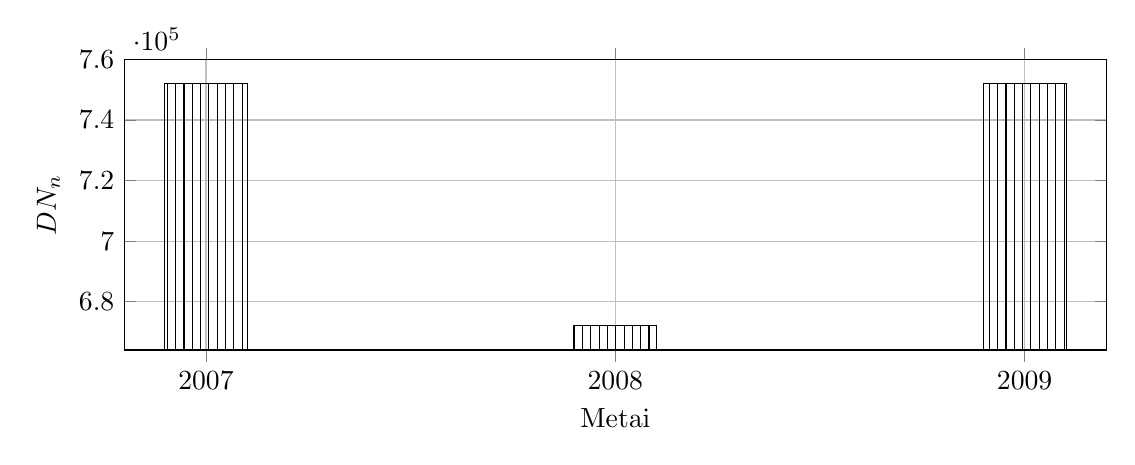
\begin{tikzpicture}
	\begin{axis}[
		x tick label style={
			/pgf/number format/1000 sep=
		},
		xtick = data,
		ybar,
		bar width=30pt,
		xlabel={Metai},
		ylabel={$DN_n$},
		width=400pt,
		height=150pt,
		grid=major,
	]
		\addplot+[draw=black, pattern=vertical lines,] coordinates {
			(2009, 7.52e5)
			(2008, 6.72e5)
			(2007, 7.52e5)
		};
	\end{axis}
\end{tikzpicture}
\end{center}
\textsf{3.1.1 pav. $DN_n$ kitimo grafikas.}\\

\begin{center}
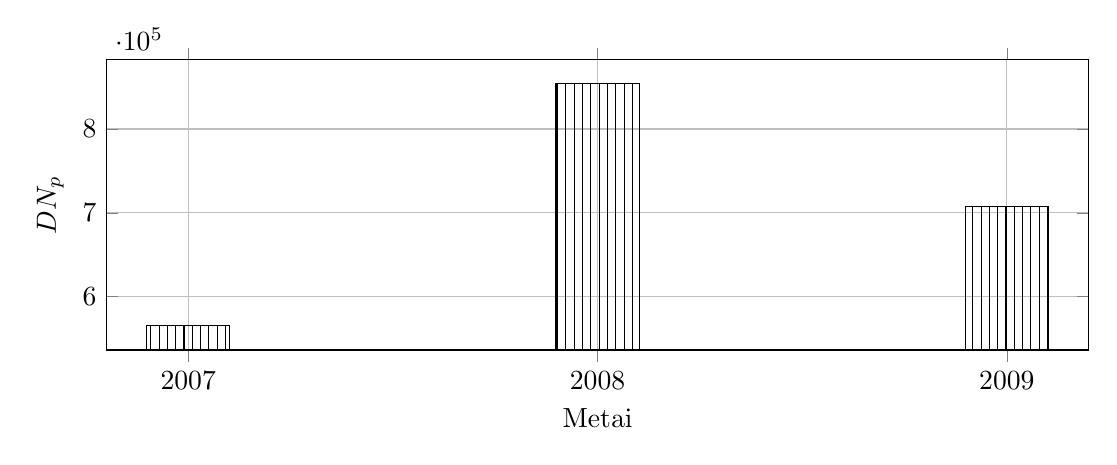
\begin{tikzpicture}
	\begin{axis}[
		x tick label style={
			/pgf/number format/1000 sep=
		},
		xtick = data,
		ybar,
		bar width=30pt,
		xlabel={Metai},
		ylabel={$DN_p$},
		width=400pt,
		height=150pt,
		grid=major,
	]
		\addplot+[draw=black, pattern=vertical lines,] coordinates {
			(2009, 707.50e3)
			(2008, 854.15e3)
			(2007, 565.14e3)
		};
	\end{axis}
\end{tikzpicture}
\end{center}
\textsf{3.1.2 pav. $DN_p$ kitimo grafikas.}\\

\begin{center}
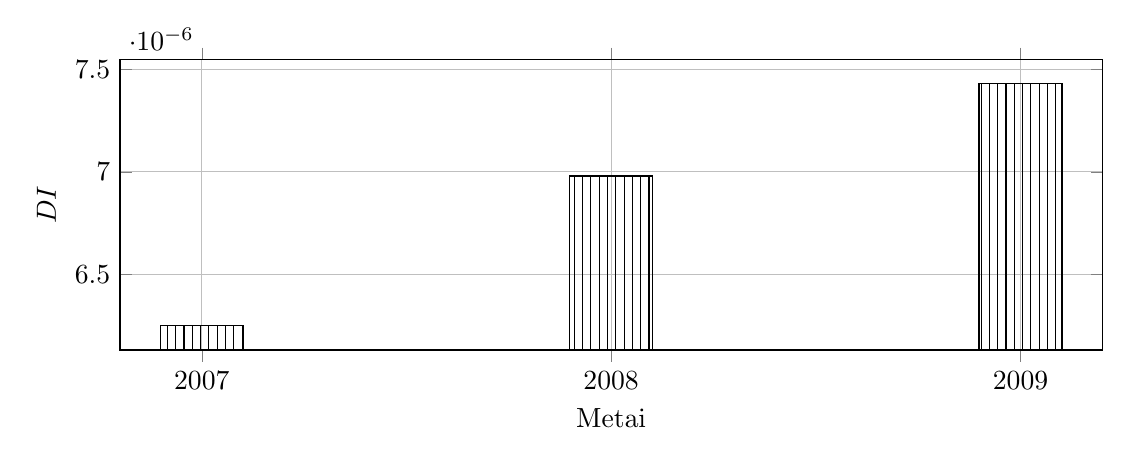
\begin{tikzpicture}
	\begin{axis}[
		x tick label style={
			/pgf/number format/1000 sep=
		},
		xtick = data,
		ybar,
		bar width=30pt,
		xlabel={Metai},
		ylabel={$DI$},
		width=400pt,
		height=150pt,
		grid=major,
	]
		\addplot+[draw=black, pattern=vertical lines,] coordinates {
			(2009, 7.43e-6)
			(2008, 6.98e-6)
			(2007, 6.25e-6)
		};
	\end{axis}
\end{tikzpicture}
\end{center}
\textsf{3.1.3 pav. $DI$ kitimo grafikas.}\\

Vidutinis vieno darbininko išdirbis (Lt arba Eurais) gali būti apskaičiuotas taip:
\begin{itemize}
	\item Vidutinis \textbf{metinis} vieno darbininko išdirbis ($I_{dnm}$):
	\[
		I_{dnm} = \frac{
			\textsf{Įmonės bendroji produkcija}
		}{
			\textsf{Vidutinis metinis sąrašinių darbininkų skaičius}
		};
	\]
	\item Vidutinis \textbf{dieninis} darbininko išdirbis ($I_{dnd}$):
	\[
		I_{dnd} = \frac{
			\textsf{Bendroji produkcija}
		}{
			\textsf{Vidutinis metinis sąrašinių darbininkų skaičius x vieno darbininko dirbtų dienų skaičius}
		}
	\]
	\item Vidutinis \textbf{valandinis} vieno darbininko išdirbis ($I_{dnv}$):
	\[
		I_{dnv} = \frac{
			\textsf{Bendroji produkcija}
		}{
			\textsf{Vsmds x Vdddpsm x Vdddt}
		}
	\]
	Kur Vmsds - Vidutinis metinis sąrašinių darbininkų skaičius, Vdddspm - Vieno darbininko dirbtų dienų skaičiaus per metus, Vdddt - Vieno darbininko darbo dienos (pamainos) trukmė.
\end{itemize}
\textsl{3.1.2 lentelė. Darbininko išdirbis.}\\
\begin{tabular}{|p{4cm}|p{4cm}|p{4cm}|p{4cm}|} \hline
	Metai & $I_{dnm}$ & $I_{dnd}$ & $I_{dnv}$ \\ \hline
	2009 	& 644.04e3 & 2.53e3 & 315.75  \\ \hline
	2008  & 671.77e3 & 2.63e3 & 329.29 \\ \hline
	2007  & 752.40e3 & 2.95e3 & 368.78 \\ \hline
\end{tabular}\\

\begin{center}
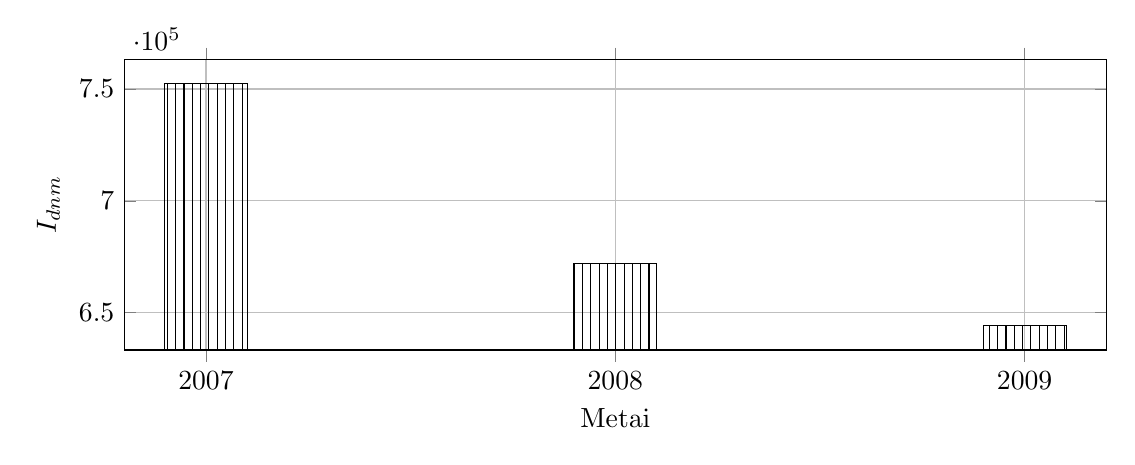
\begin{tikzpicture}
	\begin{axis}[
		x tick label style={
			/pgf/number format/1000 sep=
		},
		xtick = data,
		ybar,
		bar width=30pt,
		xlabel={Metai},
		ylabel={$I_{dnm}$},
		width=400pt,
		height=150pt,
		grid=major,
	]
		\addplot+[draw=black, pattern=vertical lines,] coordinates {
			(2009, 644.04e3)
			(2008, 671.77e3)
			(2007, 752.40e3)
		};
	\end{axis}
\end{tikzpicture}
\end{center}
\textsf{3.1.4 pav. $I_{dnm}$ kitimo grafikas.}\\

Kitų darbininko išdirbių reikšmių pokytis metų atžvilgiu lieka toks pats.\\

Darbo našumo analizėje galima pastebėti, jog natūrinio darbo našumo atžvilgiu, 
mažiausias jis buvo 2008 metais. Tuo tarpu 2007 ir 2009 jis buvo bene vienodas.
Iš piniginio darbo našumo matome, jog jis mažiausias buvo 2007 metais, padidėjo 
2008 metais ir per pus sumažėjo 2009 metais, lyginant su 2008 metais.
Darbo imlumas įmonėje per 2007-2009 metus tik didėjo.\\

Analizuodami vieno darbininko išdirbį litais, gavome, jog didžiausias jis buvo 
2007 metais, sekančiais metais smarkiai krito ( lyginant su 2007 
metais ), o 2009 metais dar labiau sumažėjo.


\subsection{Darbo struktūra}

Darbo struktūra - bendras darbininkų skaičius suskirstytas į
\begin{itemize}
	\item Vadovus
	\item Specialistus
	\item Darbininkus
\end{itemize}
\textsl{3.2.1 lentelė. Darbuotojų skaičius ir vidurinis atlyginimas 2009 metais. Duomenys 
paimti iš antro priedo.}\\
\begin{tabular}{|p{5cm}|p{5cm}|p{5cm}|} \hline
	Darbuotojai & Vidutinis sąrašinis darbuotojų skaičius & Vidutinis mėnesinis darbo užmokestis, Lt \\ \hline
	Vadovaujantysis personalas & 140 & 6866 \\ \hline
	Specialistai &	986 & 2953 \\ \hline
	Darbininkai & 661 & 2267 \\ \hline
	Iš viso:	& 1787 & 3006 \\ \hline
\end{tabular}\\\\
\textsl{3.2.2 lentelė. Darbuotojų skaičius ir vidurinis atlyginimas 2008 metais. Duomenys 
paimti iš antro priedo.}\\
\begin{tabular}{|p{5cm}|p{5cm}|p{5cm}|} \hline
	Darbuotojai & Vidutinis sąrašinis darbuotojų skaičius & Vidutinis mėnesinis darbo užmokestis, Lt \\ \hline
	Vadovaujantysis personalas & 145 & 7130 \\ \hline
	Specialistai &	959 & 2916 \\ \hline
	Darbininkai & 717 & 2243 \\ \hline
	Iš viso:	& 1821 & 2986 \\ \hline
\end{tabular}\\\\
\textsl{3.2.3 lentelė. Darbuotojų skaičius ir vidurinis atlyginimas 2007 metais. Duomenys 
paimti iš pirmo priedo.}\\
\begin{tabular}{|p{5cm}|p{5cm}|p{5cm}|} \hline
	Darbuotojai & Vidutinis sąrašinis darbuotojų skaičius & Vidutinis mėnesinis darbo užmokestis, Lt \\ \hline
	Vadovaujantysis personalas ir specialistai & 1076 & 3027 \\ \hline
	Darbininkai & 737 & 1934 \\ \hline
	Iš viso:	& 1813 & 2582 \\ \hline
\end{tabular}\\\\
Informacijos vaizdingumui, pateiksim grafikus.
\begin{center}
\begin{tikzpicture}
	\begin{axis}[
		x tick label style={
			/pgf/number format/1000 sep=
		},
		xtick = data,
		ybar,
		bar width=30pt,
		xlabel={Metai},
		ylabel={Darbuotojų skaičius},
		width=400pt,
		height=150pt,
		grid=major,
	]
		\addplot+[draw=black, pattern=vertical lines,] coordinates {
			(2009, 1787)
			(2008, 1821)
			(2007, 1813)
		};
	\end{axis}
\end{tikzpicture}
\end{center}
\textsf{3.2.1 pav. Darbuotojų skaičiaus pokytis įmonėje.}\\

\begin{center}
\begin{tikzpicture}
	\begin{axis}[
		x tick label style={
			/pgf/number format/1000 sep=
		},
		xtick = data,
		ybar,
		bar width=30pt,
		xlabel={Metai},
		ylabel={Darbuotojų atlyginimas},
		width=400pt,
		height=150pt,
		grid=major,
	]
		\addplot+[draw=black, pattern=vertical lines,] coordinates {
			(2009, 3006)
			(2008, 2986)
			(2007, 2582)
		};
	\end{axis}
\end{tikzpicture}
\end{center}
\textsf{3.2.2 pav. Darbuotojų vidutinio mėnesinio uždarbio pokytis įmonėje.}\\

Kaip matome, iš pateiktų duomenų, darbuotojų skaičius įmonėje didžiausias buvo 
2008 metais, 2009 metais darbuotojų skaičius sumažėjo. Anaiptol, darbuotojų 
vidutinis mėnesio atlyginimas nuolat didėjo. Didžiausias šuolis buvo tarp 
2007-2008 metų.

\subsection{Kapitalo struktūra}

\textsl{3.3.1 lentelė. Kapitalo struktūra. Paimta iš dviejų paskutinių priedų.}\\
\begin{tabular}{|p{5cm}|p{3cm}|p{3cm}|p{3cm}|} \hline
		& 2009 & 2008 & 2007 \\ \hline
	Kapitalas (Lt) & 1991184e3 & 1882305e3 & 1929787e3 \\ \hline
\end{tabular}\\\\

\begin{center}
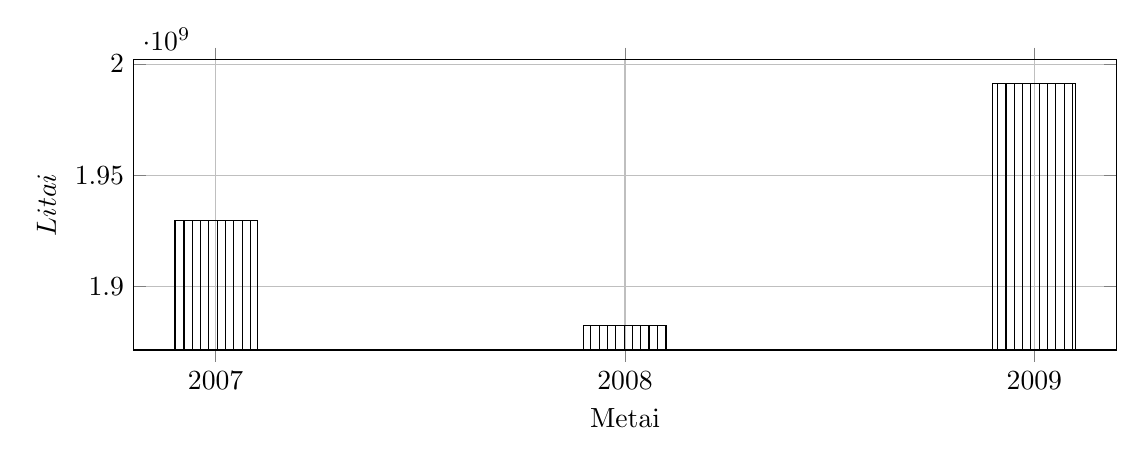
\begin{tikzpicture}
	\begin{axis}[
		x tick label style={
			/pgf/number format/1000 sep=
		},
		xtick = data,
		ybar,
		bar width=30pt,
		xlabel={Metai},
		ylabel={$Litai$},
		width=400pt,
		height=150pt,
		grid=major,
	]
		\addplot+[draw=black, pattern=vertical lines,] coordinates {
			(2009, 1991184e3)
			(2008, 1882305e3)
			(2007, 1929787e3)
		};
	\end{axis}
\end{tikzpicture}
\end{center}
\textsf{3.3.1 pav. Kapitalo struktūra.}\\

Kaip matome, įmonės kapitalas, lyginant su 2007 metais, 2008 metais sumažėjo 
daugiau negu dvigubai, o 2009 metais labai padidėjo.

\subsection{Darbo pakeitimas kapitalu}

Pakeičiamumo norma apskaičiuojama, pasitelkus sekančią formulę:
\[
	PN_n = \frac{L_{n+1}-L_n}{K_{n+1}-K_{n}};
\]
čia L - kiek atlyginimų išmokėta per metus; K - įmonės kapitalas.\\
\textsl{3.4.1 lentelė. Įmonės sumokėti atlyginimai ir kapitalas. Duomenys paimti iš keturių priedų.}\\
\begin{tabular}{|p{4cm}|p{3cm}|p{3cm}|p{3cm}|} \hline
		& 2009 & 2008 & 2007 \\ \hline
	Atlyginimai (Lt) & 5.37e6 & 5.43e6 & 4.68e6 \\ \hline
	Kapitalas (Lt) & 1991184e3 & 1882305e3 & 1929787e3 \\ \hline
\end{tabular}\\\\
\textsl{3.4.2 lentelė. Pakeičiamumo norma.}\\
\begin{tabular}{|p{4cm}|p{4cm}|} \hline
	$n$ & $PN_n$ \\ \hline
	1   & -0.015795 \\ \hline
	2   & -5.5107e-4 \\ \hline
\end{tabular}\\

Iš skaičiavimų matome, kad pakeičiamumo norma yra neigiama. Neigiamiausia jinai yra 
tarp 2007-2008 metų, o mažesnė prie 2008-2009 metų, vadinasi, įmonė juda teisinga 
linkme, siekdama didinti savo pakeičiamumo normą.

\section{Gamybos išteklių panaudojimo kryptis ir galimybės}

Planuojama, kad 2010 m. AB "Lietuvos dujos" perdavimo sistema Lietuvos vartotojams 
transportuojamų dujų kiekis sudarys apie 3 mlrd. $m^3$.\\

Per 2010 m. planuojama prijungti apie 2 tūkst. naujų vartotojų, tačiau šį skaičių 
dar gali pakoreguoti Lietuvos ekonominės situacijos pokyčiai. Bendrovės investicijos 
į naujų dujų sistemų statybą 2010 m. planuojamas didesnės nei 2009 m.\\

2010 m. planuojama baigti Jauniūnų dujų kompresorių stoties statybą. Įrengus šią stotį 
atsiras galimybė padidinti transportuojamus dujų kiekius vartotojams, padidinti 
dujų tiekimo saugumą bei patikimumą uždarius Ignalinos AE ir užtikrinti didesnį 
dujų tranzitą į Rusijos Federacijos Kaliningrado sritį. Šis projektas yra įrašytas 
į Lietuvos Nacionalinės energetikos strategijos planus.\\

Bendrovė ir toliau tęs dar iki sunkmečio pradėtus projektus, skirtus veiklos efektyvumo 
didinimui. Toliau tobulinama valdymo  struktūra, įvertinant ES teisės aktų nuostatas, 
nuosekliai vykdoma išlaidų optimizavimo politika.\\

\section*{Išvados ir pasiūlymai}
\addcontentsline{toc}{section}{Išvados ir pasiūlymai}	

AB "Lietuvos dujos" dominuoja tarp gamtinių dujų importo Lietuvoje 2009 metais. 
Krizės laikotarpiu įmonės darbuotojų skaičius ir pardavimo pajamos sumažėjo, 
bet įmonė vistiek liko dominuojančioje pozicijoje.\\

Kursinio darbo metu, susipažinau su įmonės ekonominiais analizavimo pagrindais, 
detaliau susipažinau su AB "Lietuvos dujos" valdymo struktūra, jos vizija, misija, 
jos veikla. Nors įmonės pakeičiamumo norma ir yra neigiama, tačiau neigiamas 
koeficientas mažėja, o tai rodo, kad įmonė juda teisinga linkme, norėdama 
padidinti savo pakeičiamumo normos koeficientą.\\

AB "Lietuvos dujos" nuolat tobulina savo įrangą, vykdo komercinius projektus ir 
kelia sau vis naujesnius, tolimesnius, orientuotus į ateitį, tikslus.\\

\newpage
\section*{Literatūra}
\addcontentsline{toc}{section}{Literatūra}
\begin{itemize}
	\item http://bit.ly/aKEYLL
	\item http://www.dujos.lt/index.php?item$\_$id=589
	\item http://www.dujos.lt/uploads/files/dir29/dir1/16$\_$0.php
	\item http://www.dujos.lt/uploads/files/dir17/16$\_$0.php
	\item http://www.dujos.lt/index.php/apie-mus/pagrindiniai-grupes-veiklos-rodikliai/1945
	\item Vladas Gronskas "Ekonominė analizė", "Technologija" Kaunas, 2005.
\end{itemize}
\newpage

\section*{Priedai}
\addcontentsline{toc}{section}{Priedai}
\includegraphics[width=460pt]{grupes_vidutinis_menesinis_darbo_uzmokestis_2006_2007.png}\\
\textsl{1 priedas. Grupės vidutinis mėnesio darbo užmokestis ir darbuotojų skaičius 2006-2007 metais.}\\
\includegraphics[width=460pt]{grupes_vidutinis_menesinis_darbo_uzmokestis_2008_2009.png}\\
\textsl{2 priedas. Grupės vidutinis mėnesio darbo užmokestis ir darbuotojų skaičius 2008-2009 metais.}\\
\includegraphics[width=460pt]{kapitalas_2008_2007.png}\\
\textsl{3 priedas. Grupės kapitalas 2008-2007 metais.}\\
\includegraphics[width=460pt]{kapitalas_2009_2008.png}\\
\textsl{4 priedas. Grupės kapitalas 2009-2008 metais.}\\
\end{document}
